\documentclass[a4paper,twoside,12pt]{article}
\usepackage{../z/zed-cm}
\usepackage{graphicx}
\usepackage[nottoc,numbib]{tocbibind}
\markboth{Draft}{Version 0.1}
\pagestyle{myheadings}
\begin{document}
\parskip 2 pt
\parindent 10 pt

\def\Slash{\slash\hspace{0pt}}

\title{A Container description}

\author{
Glyn Normington\and
Steve Powell
}

\maketitle
% The following three commands ensure the title page is without a page number but page numbering starts here.
% Page numbers appear on subsequent pages, and are roman until the main body, which starts again at arabic 1.
\thispagestyle{empty}
\pagenumbering{roman}
\setcounter{page}{1}

%=============================================================================

This document attempts to describe \emph{container}s (see in, for example, \cite{garden}) in a precise fashion.

% Alt-Cmd-M -- \emph{}
% Alt-Cmd-Z -- \zed{}
% Alt-Cmd-X -- \axdef{}
% Alt-Cmd-S -- \schema{}
% Alt-Shift-Cmd-T -- \texttt{}

% Type checking hacks
\newcommand{\true}{true}
\newcommand{\false}{false}
\renewcommand{\emptyset}{\varnothing}
%=============================================================================

\clearpage
\tableofcontents

\cleardoublepage
\pagenumbering{arabic}
\setcounter{page}{1}

%=============================================================================
\section{Introduction}

This is a document that records the deliberations of Glyn and Steve as they come to grips with ``what containers really
are''\footnote{``What \emph{are} containers?'' \emph{Jerzy Czaykowski} (adapted)}.

%=============================================================================
\section{Overview of this document}

This document is a rag-bag of concepts and ideas (at the moment). The intention is to find the right decomposition of ideas to simply describe the state, and state transitions, of \emph{Containers} and the \emph{Jobs} that they \emph{Run}.

%=============================================================================
\section{Containers}

\begin{schema}{MultiSS}
dummy : \nat
\end{schema}

\begin{zed}
[FILESYSTEM, NETWORK, PID, TASK]
\end{zed}

\begin{schema}{Job}
t: TASK\\
\end{schema}

\begin{zed}
ContainerState ::= STARTED | STOPPED
\end{zed}


\begin{schema}{Container}
fs : FILESYSTEM \\
network : NETWORK \\
MultiSS\\
jobs : PID \pfun Job \\
state : ContainerState \\

\end{schema}

%=============================================================================
\section{Initial whiteboard stuff}

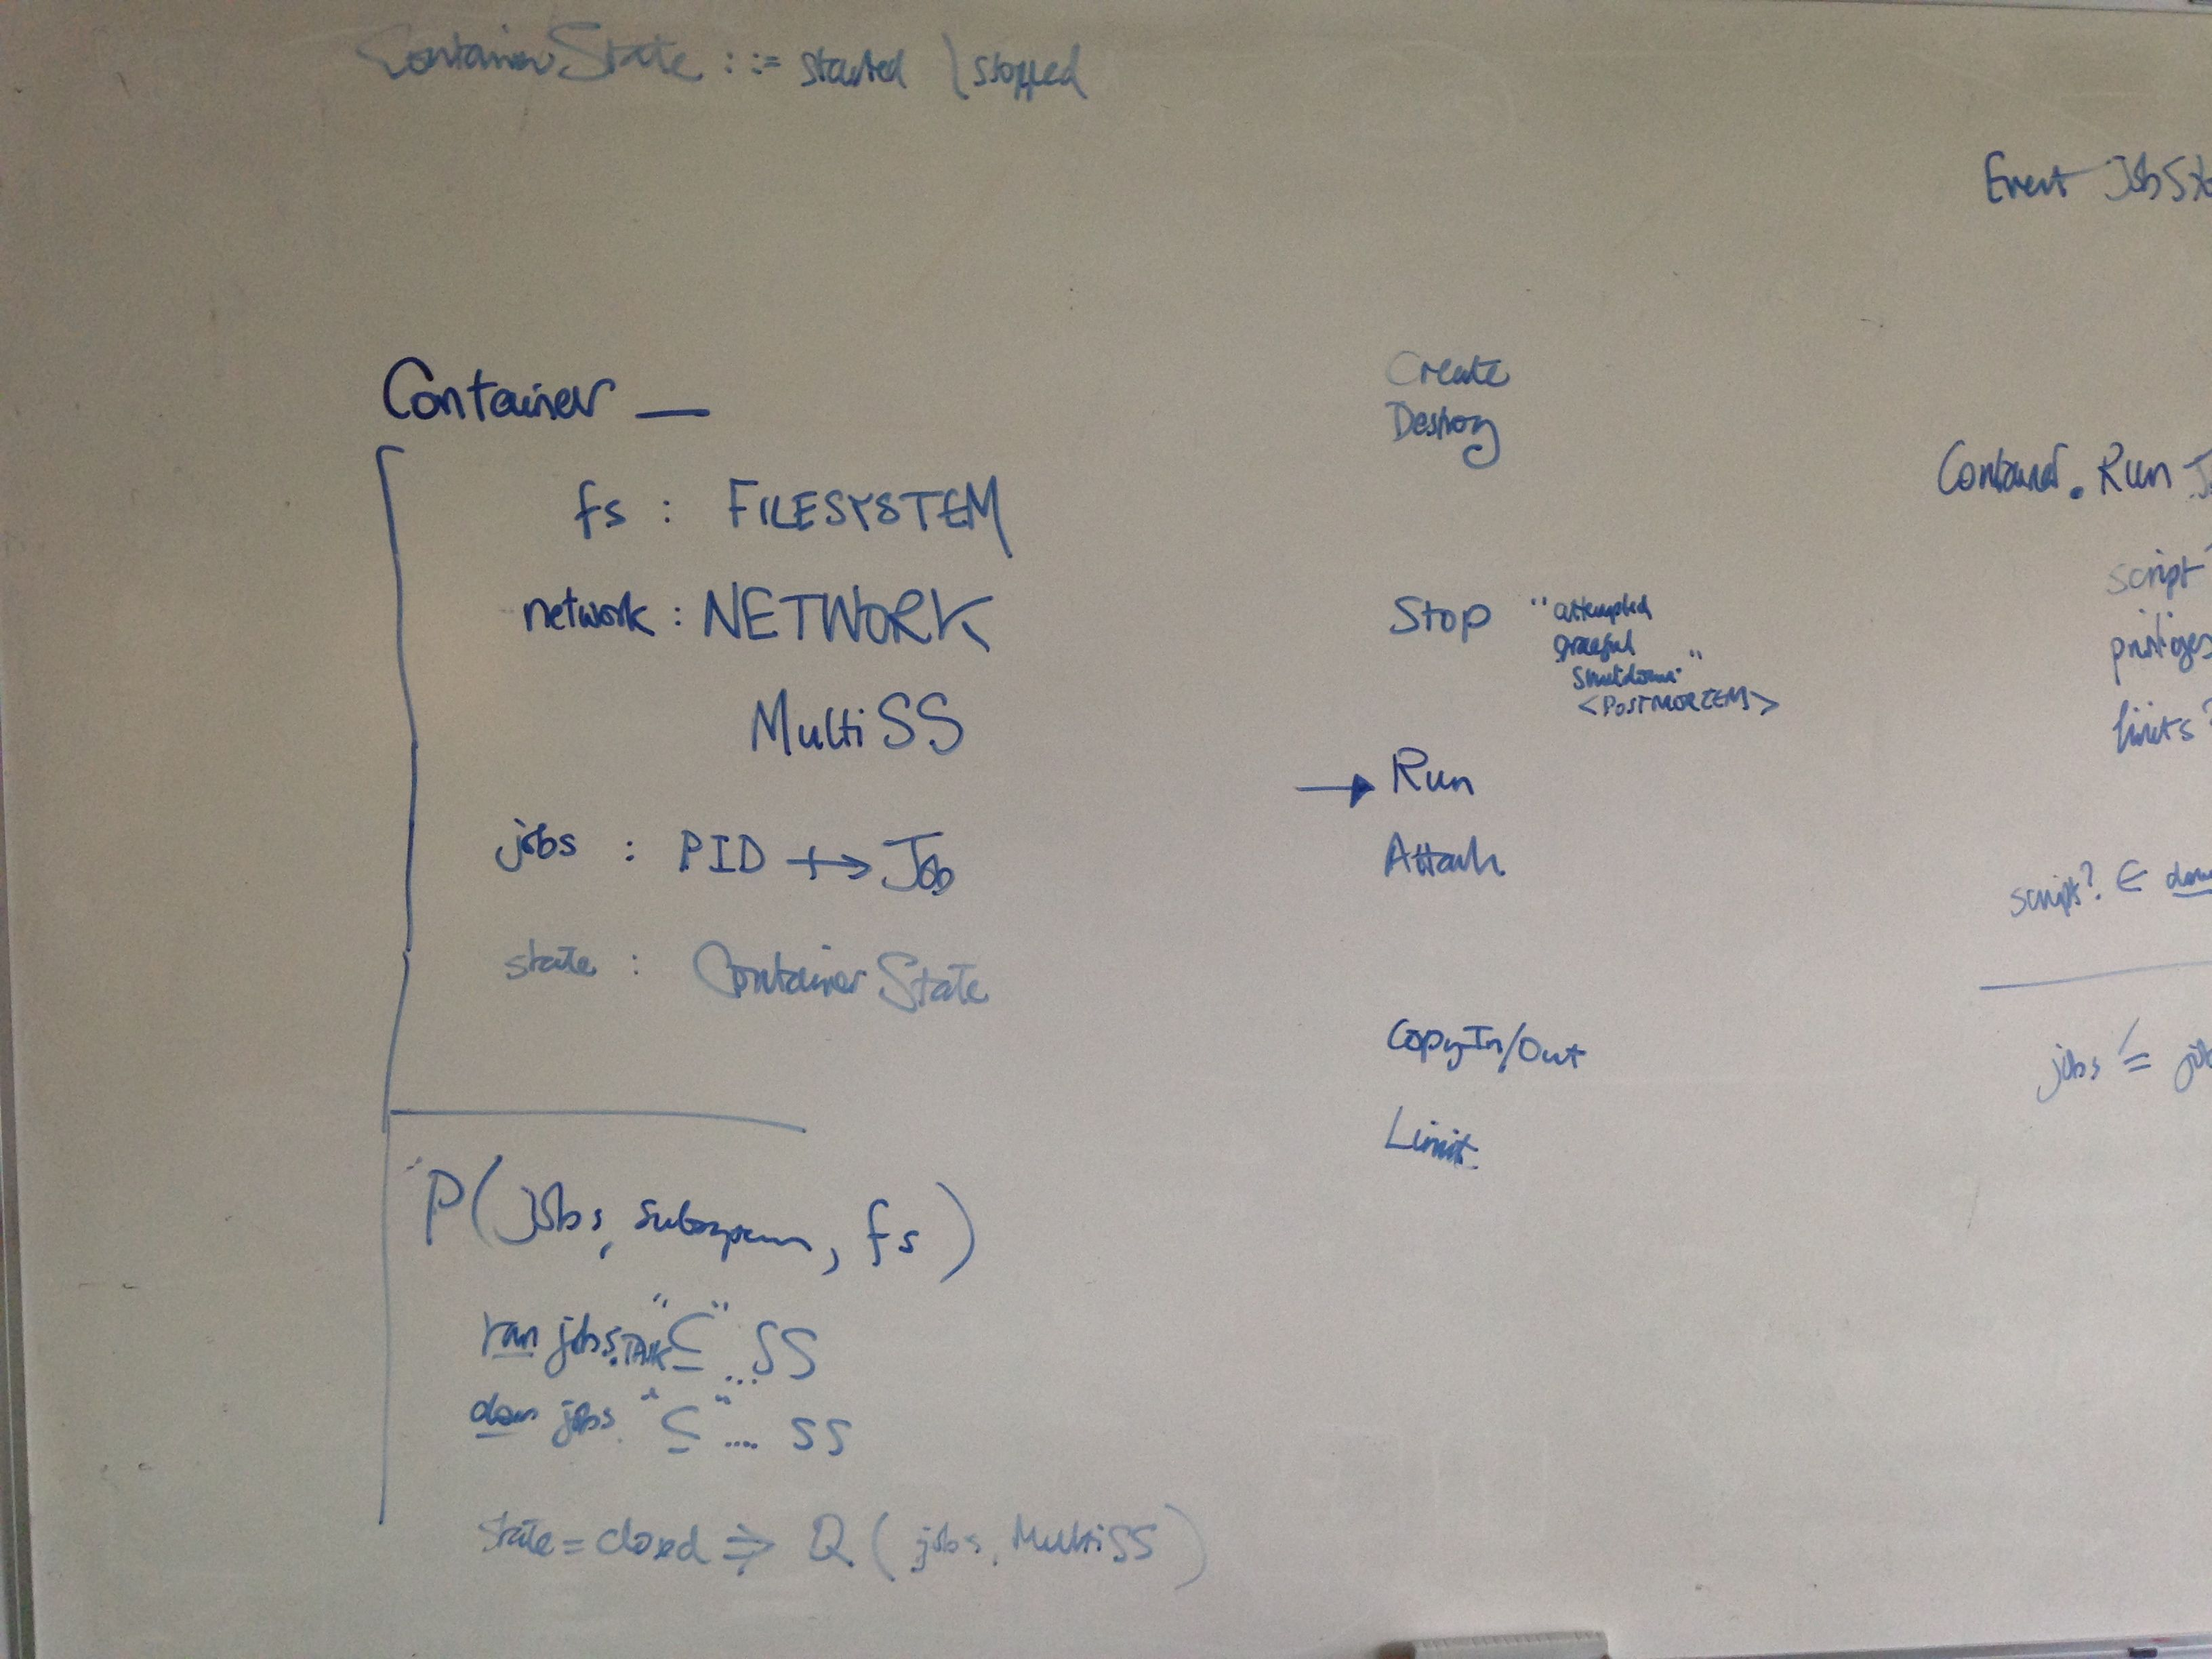
\includegraphics[width=0.9\textwidth]{pics/IMG_0685.jpg}

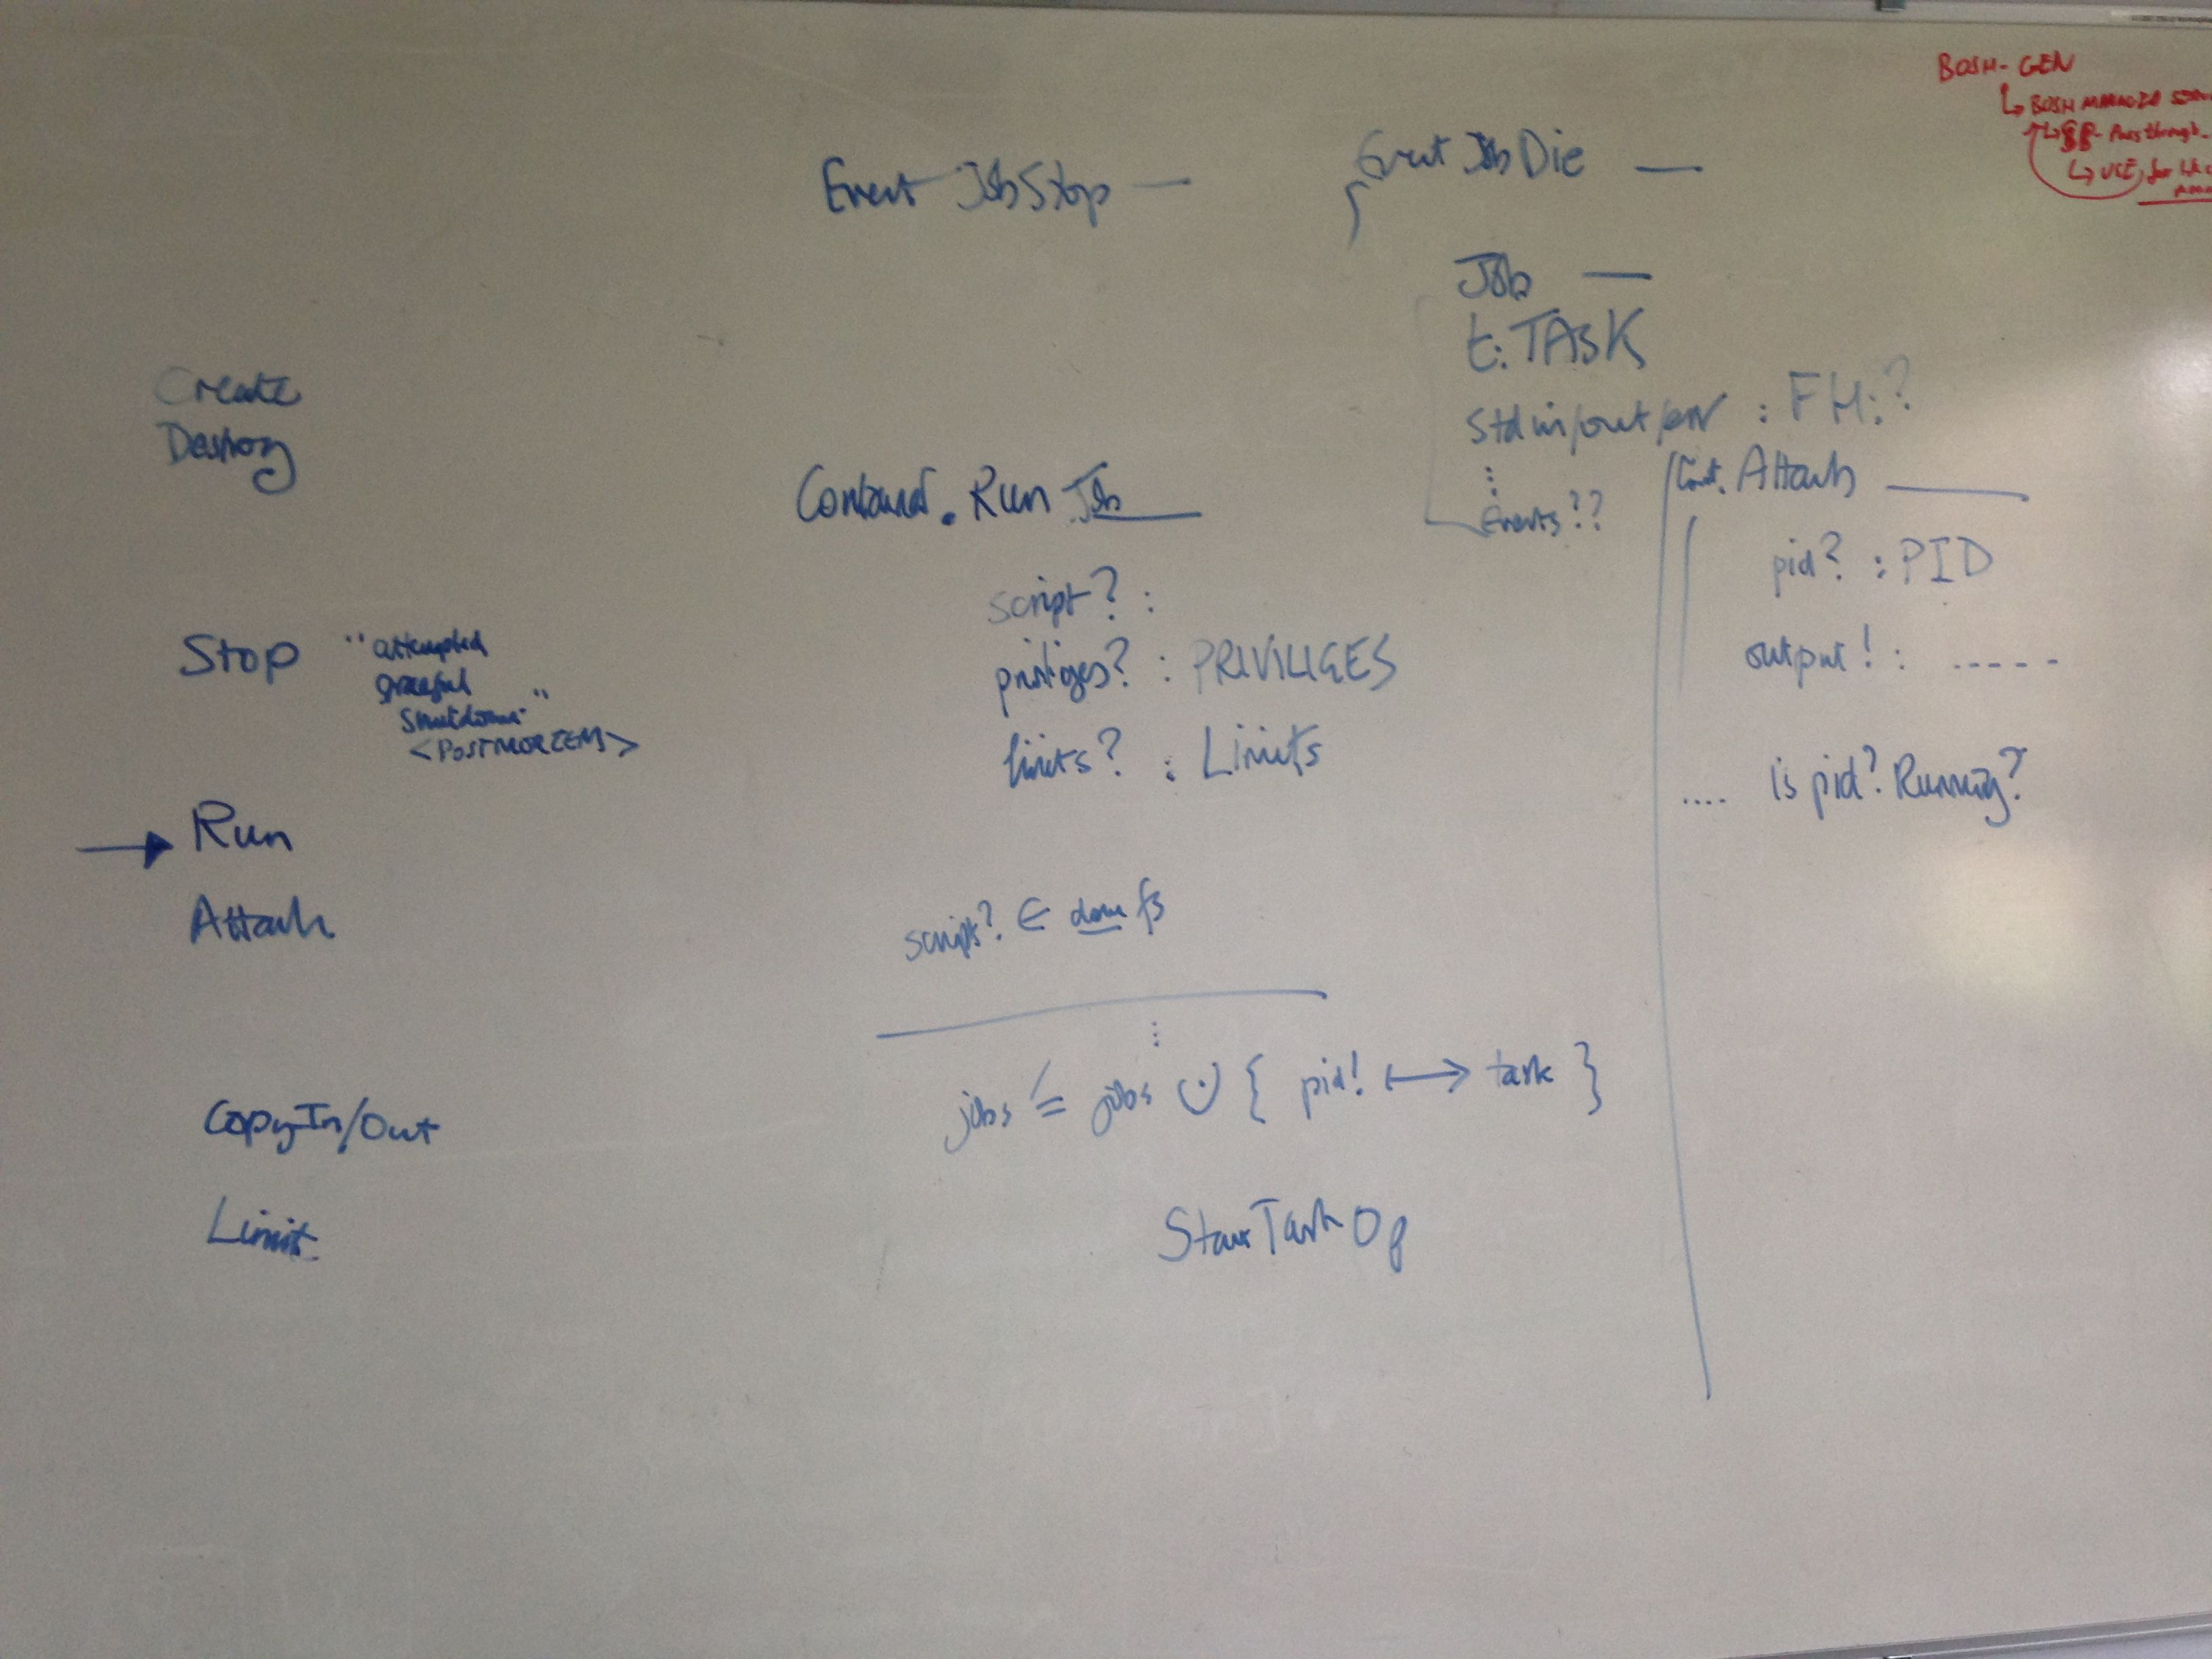
\includegraphics[width=0.9\textwidth]{pics/IMG_0686.jpg}


%%%%%%%%%%%%%%%%%%%%%%%%%%%%%%%%%%%%%%%%%%%%%%%
%   A P P E N D I C E S
%%%%%%%%%%%%%%%%%%%%%%%%%%%%%%%%%%%%%%%%%%%%%%%

\clearpage

\appendix

%=============================================================================
%   Z   N O T A T I O N
%=============================================================================
\section{Z Notation}
\label{sec:znot}
{\scriptsize
\makeatletter % the following code is taken from Mike Spivey's zed.tex

\def\symtab{\setbox0=\vbox\bgroup \def\\{\cr}
        \halign\bgroup\strut$##$\hfil&\quad##\hfil\cr}
\def\endsymtab{\crcr\egroup\egroup
        \dimen0=\ht0 \divide\dimen0 by2 \advance\dimen0 by\ht\strutbox
        \splittopskip=\ht\strutbox \vbadness=10000
        \predisplaypenalty=0
        $$\halign{##\cr\hbox to\linewidth{%
                \valign{##\vfil\cr
                        \setbox1=\vsplit0 to\dimen0 \unvbox1\cr
                        \noalign{\hfil}\unvbox0\cr
                        \noalign{\hfil}}}\cr
                \noalign{\prevdepth=\dp\strutbox}}$$
        \global\@ignoretrue}

\makeatother

Numbers:
\begin{symtab}
        \nat & \verb/Natural numbers/ \{\verb/0,1,.../\} \\
%       \num & \verb/Integers (...,-1,0,1,...)/ \\
%       \nat_1 & \verb/Positive natural numbers/ \\
%       \upto & \verb/integral range/ \\
%       + & \verb/Addition/\quad\hfill 3 \\
%       - & \verb/Subtraction/\quad\hfill 3 \\
%       * & \verb/Multiply/\quad\hfill 4 \\
%       \div & \verb/Remainder/\quad\hfill 4 \\
%       \mod & \verb/Modulus/\quad\hfill 4 \\
%       < & \verb/Less than/ \\
%       > & \verb/Greater than/ \\
%       \leq & \verb/Less than or equal/ \\
%       \geq & \verb/Greater than or equal/ \\
%       \neq & \verb/Inequality/ \\
\end{symtab}
Propositional logic and the schema calculus:
\begin{symtab}
%       \lnot & \verb/Not/ \\
        \ldots\land\ldots & \verb/And/ \\
        \ldots\lor\ldots & \verb/Or/ \\
        \ldots\implies\ldots & \verb/Implies/ \\
%       \iff & \verb/If and only if/ \\
        \forall..\mid..\spot.. & \verb/For all/ \\
        \exists..\mid..\spot.. & \verb/There exists/ \\
%       \exists_1..\mid..\spot.. & \verb/There exists unique/ \\
        \ldots\hide\ldots & \verb/Hiding/ \\
%       \project & \verb/\project/ \\
%       \pre & \verb/\pre/ \\
%       \semi & \verb/\semi/
        \ldots\defs\ldots & \verb/Schema definition/ \\
        \ldots==\ldots & \verb/Abbreviation/ \\
        \ldots::=\ldots\mid\ldots & \verb/Free type definition/ \\
        \ldata\ldots\rdata & \verb/Free type injection/ \\
        [\ldots] & \verb/Given sets/ \\
        ',?,!,_0\ldots_9 & \verb/Schema decorations/ \\
        \ldots\shows\ldots & \verb/theorem/ \\
        \theta\ldots & \verb/Binding formation/ \\
        \lambda\ldots & \verb/Function definition/ \\
        \mu\ldots & \verb/Mu-expression/ \\
        \Delta\ldots & \verb/State change/ \\
        \Xi\ldots & \verb/Invariant state change/ \\
\end{symtab}
Sets and sequences:
%and bags:
\begin{symtab}
        \{\ldots\} & \verb/Set/ \\
        \{..\mid..\spot..\} & \verb/Set comprehension/ \\
        \power\ldots & \verb/Set of subsets of/ \\
%       \power_1 & \verb/Non-empty subsets of/ \\
%       \finset & \verb/Finite sets/ \\
%       \finset_1 & \verb/Non-empty finite sets/ \\
        \emptyset & \verb/Empty set/ \\
        \ldots\cross\ldots & \verb/Cartesian product/ \\
        \ldots\in\ldots & \verb/Set membership/ \\
        \ldots\notin\ldots & \verb/Set non-membership/ \\
        \ldots\cup\ldots & \verb/Union/ \\
        \ldots\cap\ldots & \verb/Intersection/ \\
        \ldots\setminus\ldots & \verb/Set difference/ \\
        \bigcup\ldots & \verb/Distributed union/ \\
%       \bigcap & \verb/Distributed intersection/ \\
        \#\ldots & \verb/Cardinality/ \\
%       \dcat & \verb/Distributed sequence concatenation/
        \ldots\subseteq\ldots & \verb/Subset/ \\
        \ldots\subset\ldots & \verb/Proper subset/ \\
        \ldots\partition\ldots & \verb/Set partition/ \\
        \seq & \verb/Sequences/ \\
%       \seq_1 & \verb/Non-empty sequences/ \\
%       \iseq & \verb/Injective sequences/ \\
        \langle\ldots\rangle & \verb/Sequence/ \\
%       \cat & \verb/Sequence concatenation/ \\
        \disjoint\ldots & \verb/Disjoint sequence of sets/ \\
%       \bag & \verb/Bags/ \\
%       \lbag\ldots\rbag & \verb/Bag/ \\
%       \inbag & \verb/Bag membership/ \\
\end{symtab}
%Here are the infix function symbols. Each symbol is
%shown with its priority:
%\begin{symtab}
%       \uplus & \verb/\uplus/ \\
%       \filter & \verb/Schema projection/ \\
%       \uminus & \verb/\uminus/
%\end{symtab}
Functions and relations:
\begin{symtab}
        \ldots\rel\ldots\quad\quad~~~  & \verb/Relation/ \\
        \ldots\pfun\ldots & \verb/Partial function/ \\
        \ldots\fun\ldots  & \verb/Total function/ \\
        \ldots\pinj\ldots & \verb/Partial injection/ \\
        \ldots\inj\ldots  & \verb/Injection/ \\
%       \psurj & \verb/Partial surjection/ \\
%       \surj & \verb/Surjection/ \\
%       \bij  & \verb/Bijection/ \\
%       \ffun & \verb/Finite partial function/ \\
%       \finj & \verb/Finite partial injection/ \\
        \dom\ldots & \verb/Domain/ \\
        \ran\ldots & \verb/Range/ \\
        \ldots\mapsto\ldots & \verb/maplet/ \\
        \ldots\inv & \verb/Relational inverse/ \\
%       \ldots\plus & \verb/Transitive closure/ \\
        \ldots\star & \verb/Reflexive-transitive/ \\
        ~           & \verb/closure/ \\
%       \ldots\bsup n \esup & \verb/Relational iteration/ \\
        \ldots\limg\ldots\rimg & \verb/Relational image/ \\
%       \comp & \verb/Forward relational composition/ \\
%       \circ & \verb/Relational composition/ \\
        \ldots\oplus\ldots & \verb/Functional overriding/ \\
        \ldots\dres\ldots & \verb/Domain restriction/ \\
        \ldots\rres\ldots & \verb/Range restriction/ \\
        \ldots\ndres\ldots & \verb/Domain subtraction/ \\
        \ldots\nrres\ldots & \verb/Range subtraction/ \\
%       \id & \verb/Identity relation/ \\
\end{symtab}
Axiomatic descriptions:
%%unchecked
\begin{axdef}
  Declarations
\where
  Predicates
\end{axdef}
Schema definitions:
%%unchecked
\begin{schema}{SchemaName}
  Declaration
\where
  Predicates
\end{schema}
}
\newpage

%=============================================================================
%   B I B L I O G R A P H Y
%=============================================================================
\newpage
\begin{flushleft}
\begin{thebibliography}{99}
\label{sec:references}
% `99' is a picture of the generated numeric references -- they are two digits in this bibliography
% If we had a hundred or more we would have used 999, or whatever.

%%  Example bibliography entry:
%\bibitem{knuth76}                                                        % citation callout, e.g.: \cite{knuth76}
%  Donald E. Knuth,                                                        % author
%  \emph{The computer as Master Mind}.                    % title
%  J. Recreational Mathematics, Vol.~9(1), 1976-1977. % publisher, or journal, volume and date

\bibitem{warden}
  Various authors,
  \emph{Warden github repository},
  \texttt{https://github.com/cloudfoundry/warden}.

\bibitem{garden}
  Various authors,
  \emph{Garden github repository},
  \texttt{https://github.com/pivotal-cf-experimental/garden}.

% API abstracting the cgroup filesystem
% See http://manpages.ubuntu.com/manpages/lucid/man5/cgconfig.conf.5.html for configuration containing useful insights
\bibitem{libcgroup}
  Various authors
  \emph{libcgroup},
  {\small \texttt{http://libcg.sourceforge.net/html/index.html}}.

\bibitem{linuxgroups}
  Paul Menage, Paul Jackson and Christoph Lameter,
  \emph{CGROUPS},
  {\small \texttt{https://www.kernel.org/doc/Documentation/cgroups/cgroups.txt}}, 2004-2006.

\bibitem{linuxkernel}
  Linus Torvalds, \emph{et al},
  \emph{Linux kernel source tree},
  {\small \texttt{https://github.com/torvalds/linux}}.

\bibitem{memory}
  Various authors,
  \emph{Memory Resource Controller},
  {\small \texttt{https://www.kernel.org/doc/Documentation/cgroups/memory.txt}}.

\bibitem{noop}
  Kamezawa Hiroyuki, \emph{et al},
  \emph{NOOP cgroup subsystem},
  {\small \texttt{http://thread.gmane.org/gmane.linux.kernel/777763}}.

\bibitem{rharticle}
  Martin Prpi\u{c}, R\"udiger Landmann, and Douglas Silas,
  \emph{Red Hat Enterprise Linux 6.5 GA: Resource Management Guide},
  {\small \texttt{https://access.redhat.com/site/documentation/en-US\slash{}Red\_Hat\_Enterprise\_Linux/6/pdf/Resource\_Management\_Guide\slash{}Red\_Hat\_Enterprise\_Linux-6-Resource\_Management\_Guide-en-US.pdf}}.

\bibitem{7sins}
  Bertrand Meyer,
  \emph{On Formalism In Specifications},
  IEEE Software, Vol.~2(1), 1985.
\end{thebibliography}
\end{flushleft}
\end{document}
